% ! TeX root = ../../main.tex
\chapter{Design e tecnologie}
\section{Obiettivo}
L'obiettivo di questo progetto è sviluppare un app mobile per smartphone che mostri agli utenti quanto tramite risparmio di carta è possibile risparmiare grandi quantità di carta che corrisponde a co2 non emessa nell'ambiente. L'app tramite AR 
\section{Requisiti e analisi}
\subsection{Requisiti funzionali}
\subsubsection{App mobile}
% \begin{itemize}
%     \item L'app deve presentare una schermata che raggruppi tutti gli alberi collezionati dall'utente e dei relativi progetti UniBo associati. Per ciascun elemento si deve mostrare una descrizione e dettagli sui risparmi ottenuti in diverse unità di misura.
%     \item La scansione di un albero deve essere avviabile in qualsiasi momento all'interno dell'app. Dopo l'identificazione di un albero si deve avviare la modalità di realtà aumentata dove vengono mostrati i plichi di carta e le taniche di benzina risparmiate. Inoltre deve essere presente una sezione con le informazioni sull'albero e sul progetto associato. L'albero identificato, se non già presente, viene aggiunto alla collezione dell'utente.
%     \item Ogni albero nuovo aggiunto alla collezione dovrà sbloccare un badge e aumentare il livello dell'utente.
%     \item I progressi utente dovranno essere mostrati in una pagina dedicata. Nello specifico dovranno essere mostrati il livello, i badge e dei contatori sul risparmio raggiunto con la collezione personale di alberi. Dovrà essere presente anche una sezione che mostri le informazioni personali (es. nome, congome), di carriera (es. corso, anno immatricolazione) e una foto. Tutte queste informazioni dovranno essere modificabili.
%     \item L'utente deve poter condividere i progressi raggiunti accedendo ad una pagina dedicata dove verrà chiesto di scansionare il codice QR identificativo del totem.
% \end{itemize}
\subsubsection{Totem}
\begin{itemize}
    \item Devono essere presenti le schermate: homepage, statistiche, classifica e informazioni.
    \item Condivisione progressi: l'utente deve poter depositare i progressi raggiunti in app in qualsiasi momento indipendentemente dalla schermata del totem. Deve quindi essere sempre accessibile il codice QR che identifica il totem in modo da poterlo scansionare tramite app.
    \item La homepage deve mostrare gli utenti coinvolti e i dettagli dei loro progressi depositati.
    \item La schermata delle statistiche deve mostrare il conteggio totale di alberi e progetti coinvolti, la carta, l'elettricità, la benzina, la corrente elettrica e la co2 virtualmente risparmiata con la partecipazione degli utenti. Si deve mostrare una breve descrizione per ciascun dato mostrato.
    \item La classifica deve mostrare i 10 migliori utenti che hanno partecipato sulla base della co2 risparmiata.
    \item Nella pagina delle informazioni deve essere presente la spiegazione dei calcoli fatti per i dati mostrati nelle altre schermate e una sezione con maggiori dettagli sul progetto a cui fa riferimento l'esperienza sostenibile. Deve essere possibile integrare ed aggiungere nuove sezioni.
\end{itemize}
\subsection{Requisiti non funzionali}
\subsubsection{App mobile}
\subsubsection{Totem}
\begin{itemize}
    \item Il sistema deve essere scalabile in modo da permettere l'aggiunta di nuovi totem interattivi e gestire simultaneamente più richieste di condivisione dei dati dall'applicazione.
    \item L'interfaccia deve apparire familiare ed intuitiva, in modo da permettere un utilizzo immediato e non scoraggiare gli utenti all'interazione.
    \item La sincronizzazione dei dati deve essere, per quanto possibile, immediata in modo da mostrare sempre dati aggiornati.
\end{itemize}

\subsection{Modello del dominio}

%
%
%
%
\section{Design}
\subsection{Architettura}
Il sistema si compone di tre componenti principali: l'app mobile, il totem e il database cloud.

La condivisione dei progressi dell'utente dall'app al totem avviene passando per il database cloud Firebase Realtime in cui vengono memorizzati i dati.
In figura \ref{fig:communication-schema} viene mostrato uno schema delle interazioni fra i tre componenti del sistema: i progressi dell'utente vengono prima caricati sul database nel cloud quindi successivamente scaricati sul totem.
Oltre ai dati condivisi degli utenti, il database online fornisce le informazioni sugli alberi e i progetti corrispondenti sia al totem che all'app mobile.
\begin{figure} [h]
    \centering
    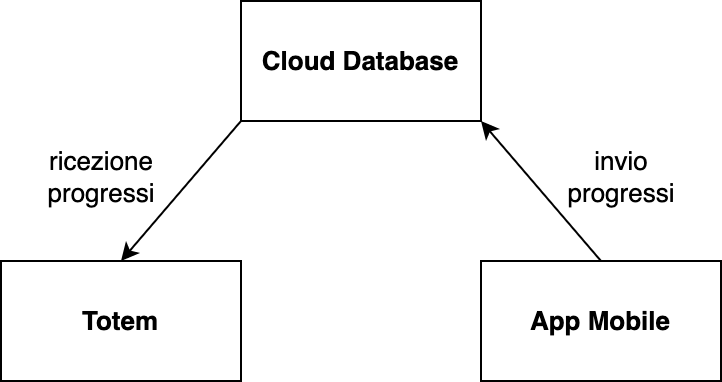
\includegraphics[width=0.5\textwidth]{img/arch-totem-app-dati.png}
    \caption{Schema della architettura e interazione fra app e totem}
    \label{fig:communication-schema}
\end{figure}
% MVVM model-viewmodel-view (utilizza il Provider Pattern per non dover passare il viewmodel nella gerarchia) nella app, potrebbe anche essere pattern DAO anche se questo non prevede una view
% Singleton pattern to manage the instance of a database connection or an HTTP client.

\subsection{Mockup}
Attraverso i \textit{mockup}, vengono presentate e spiegate le diverse schermate del totem.
Il termine \textit{mockup} o \textit{mock-up}, in italiano \enquote*{modello}, è una realizzazione a scopo illustrativo o espositivo di un oggetto o sistema, senza le complete funzioni dell'originale. Viene tipicamente sviluppato per fornire un'idea visiva del prodotto finale ai clienti, permettendo di effettuare correzioni o modifiche sulla bozza del prodotto ancora prima che si passi alla fase di sviluppo.

Per la creazione dei mockup è stato utilizzato il software Figma anche se in commercio ne esistono molti altri come ad esempio Adobe XD o Balsamiq.

Lo sviluppo della UI ha richiesto l'adattamento e la semplificazione degli elementi grafici in modo da semplificare l'interazione dell'utente con il totem rendendola il più intuitiva possibile. Vengono mantenuti i colori e il dettaglio dell'erba (figura \ref{fig:grassDetails}) dell'app mobile.

\begin{figure}
    \centering
    
\includegraphics[width=0.4\textwidth]{img/grassDetail.png}
    \caption{Dettaglio dell'erba presente nella'app e nel totem}
    \label{fig:grassDetails}
\end{figure}

\subsubsection{Mobile app}


\subsubsection{Totem}
La struttura dell'interfaccia del totem si suddivide in due sezioni principali: una colonna a sinistra contenente la barra di navigazione e la sezione con il QR code del totem e lo spazio restante a destra dove viene visualizzata la pagina selezionata (figura \ref{fig:viewStruct}).
\begin{figure}[h]
    \centering
    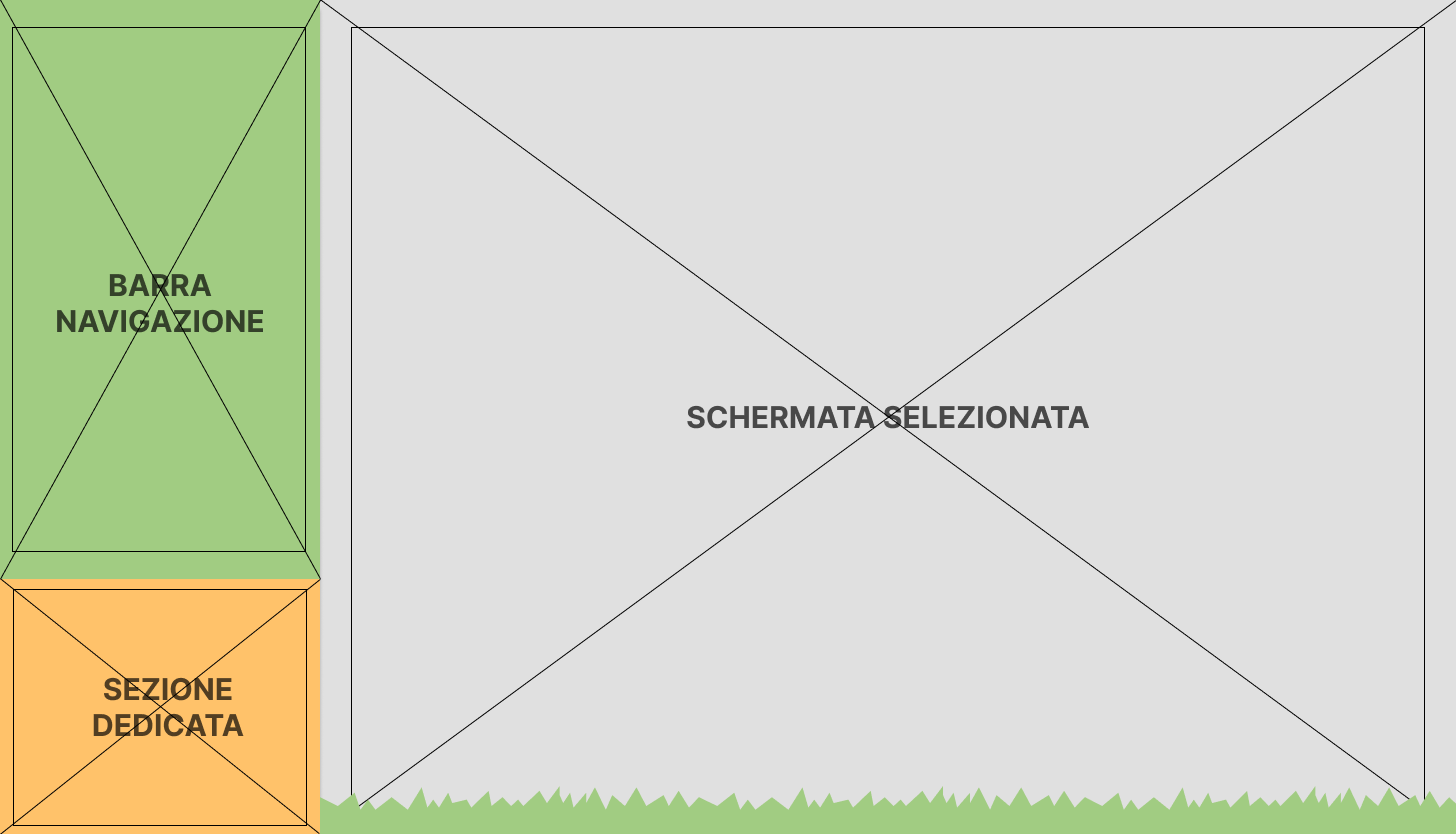
\includegraphics[width=0.8\textwidth]{img/mainStructure.png}
    \caption{Layout generale della UI del totem composto da tre blocchi: barra di navigazione (in verde), sezione codice QR (in arancione) e schermata selezionata (in grigio)}
    \label{fig:viewStruct}
\end{figure}

Di seguito si mostrano i mockup della homepage (fig. \ref{fig:homepages}), statistiche (fig. \ref{fig:statsPage}), classifica (fig. \ref{fig:chartPage}) e informazioni (fig. \ref{fig:infoPage}).

% % \subsubsection{Sezione dedicata al QR code del totem}
% In questa sezione deve essere mostrato il codice QR che identifica il totem e si è deciso di renderlo visibile solo su richiesta esplicita dell'utente.
% In figura \ref{fig:depositIconsQR} viene mostrata l'icona del pulsante. Si compone di due immagini: un vaso ed una freccia verde (figura \ref{fig:hideQR}). Al tocco del pulsante la freccia svanisce, il vaso si ingrandisce fino a contenere al suo interno il codice QR (figura \ref{fig:showQR}).

% \begin{figure} [h]
%     \centering
%     \subfloat[Codice QR del totem nascosto]{
%         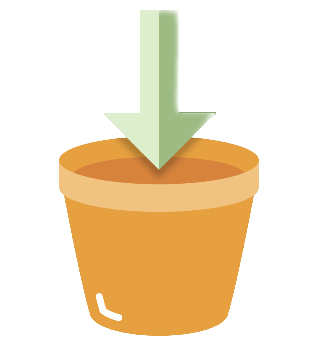
\includegraphics[width=4cm]{img/depositIcon.png}
%         \label{fig:hideQR}
%     }
%     \vspace{1cm}
%     \subfloat[Codice QR del totem visibile]{
%         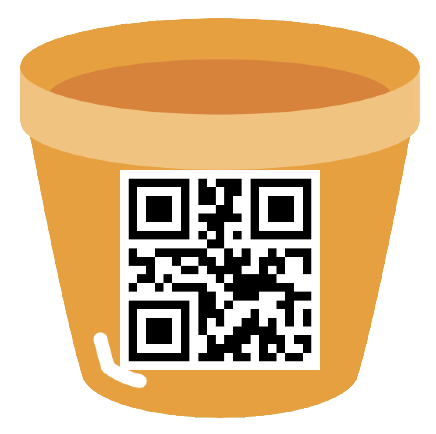
\includegraphics[width=4cm]{img/depositQR.png}
%         \label{fig:showQR}
%     }
%     \caption{Pulsante per mostrare e nascondere il codice QR identificativo del totem per la condivisione dei dati da APP}
%     \label{fig:depositIconsQR}
% \end{figure}

Per quanto riguarda la homepage sono stati fatti due mockup con design differenti: nel primo vengono mostrati gli utenti come piccoli alberi disposti su delle mensole (figura \ref{fig:shelfHome}), nel secondo viene utilizzato un layout a griglia e gli utenti vengono rappresentati come chiome di alberi visti dall'alto (figura \ref{fig:forestHome}). In entrambi i casi il tocco di un elemento espande il pannello dei dettagli utente e le chiome e alberi variano in base al livello raggiunto.

\begin{figure}[h]
    \centering
    \subfloat[Visualizzazione a mensole]{
        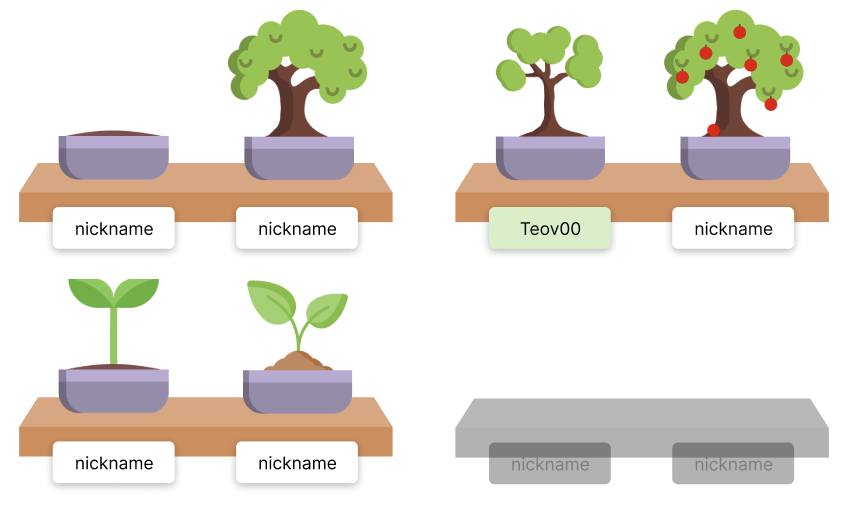
\includegraphics[width=0.45\textwidth]{img/shelfViewHome.png}
        \label{fig:shelfHome}
    }
    \subfloat[Visualizzazione a bosco]{
        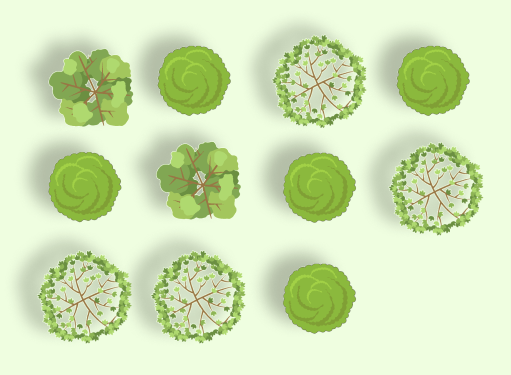
\includegraphics[width=0.45\textwidth]{img/forestViewHome.png}
        \label{fig:forestHome}
    }
    \caption[Alternative di homepage nel totem]{Design alternativi per la homepage del totem}
    \label{fig:homepages}
\end{figure}

Nella homepage è presente un pannello a scomparsa che mostra i dettagli dell'utente selezionato. Sono stati pensati quattro diversi temi:
%TODO: MENO PIPPONI E AGGIUNGERE quello con particolare tondeggiante (da notability appunti)
\begin{figure}[h]
    \centering
    \subfloat[Stile mensola]{
        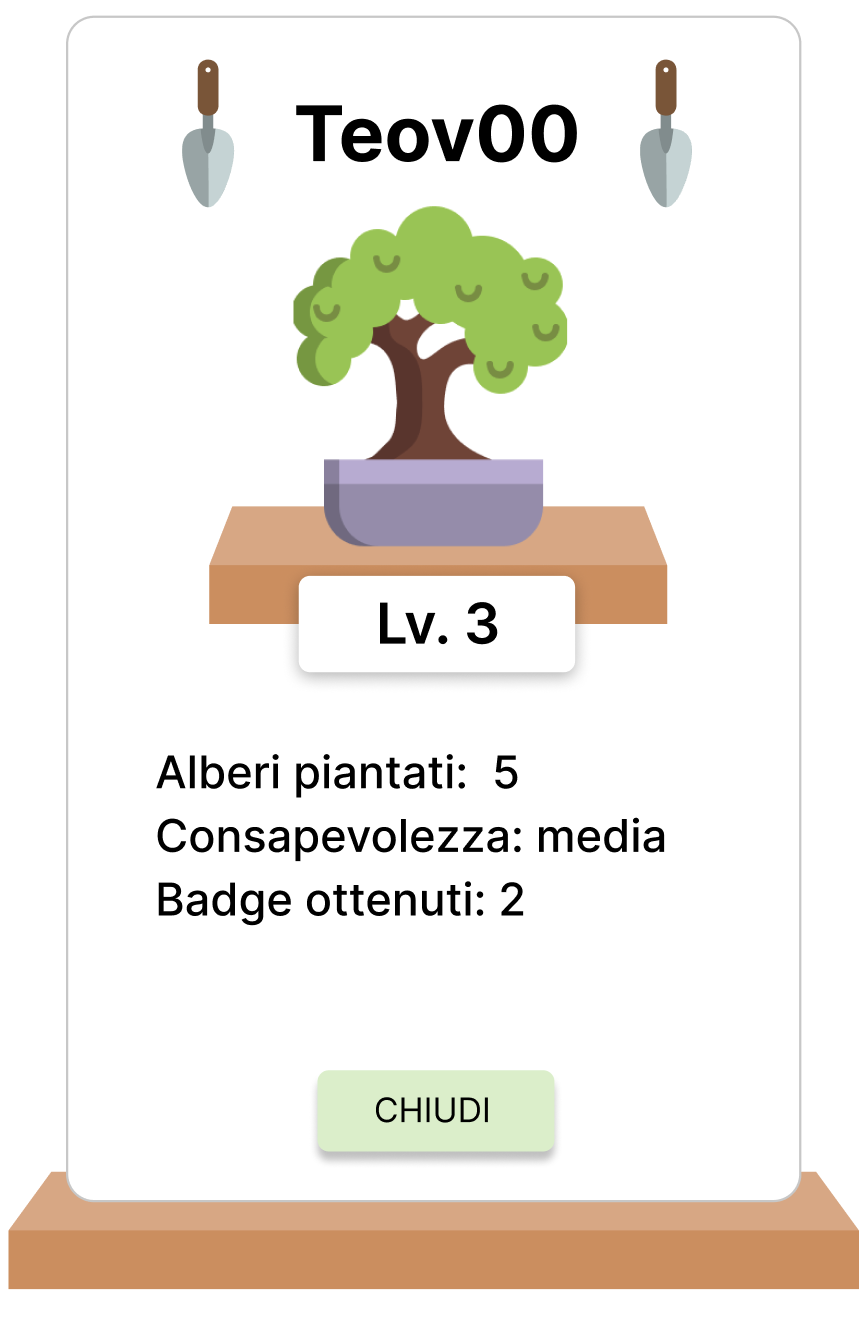
\includegraphics[width=0.30\textwidth]{img/shelfDetail.png}
        \label{fig:shelfDetail}
    }
    \subfloat[Stile tendina]{
        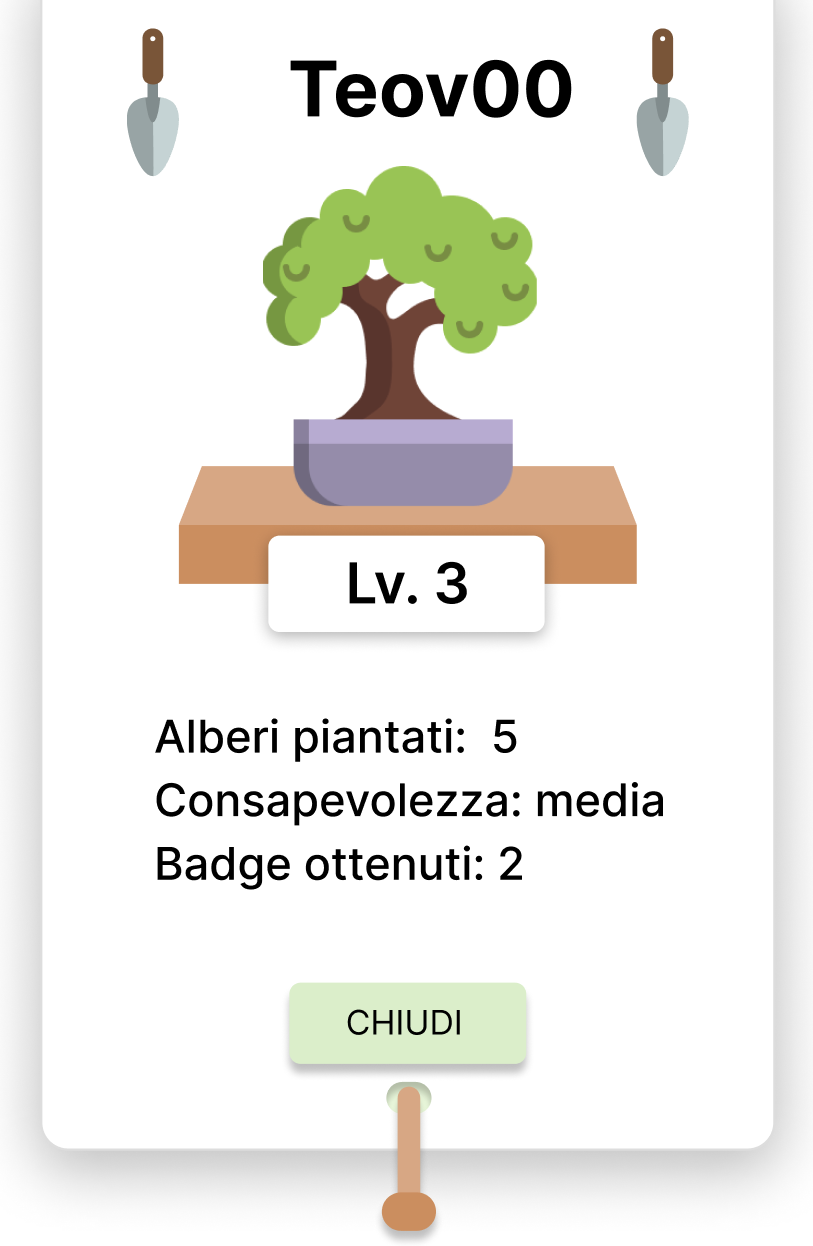
\includegraphics[width=0.30\textwidth]{img/cordDetail.png}
        \label{fig:cordDetail}
    }
    \subfloat[Stile rettangolo]{
        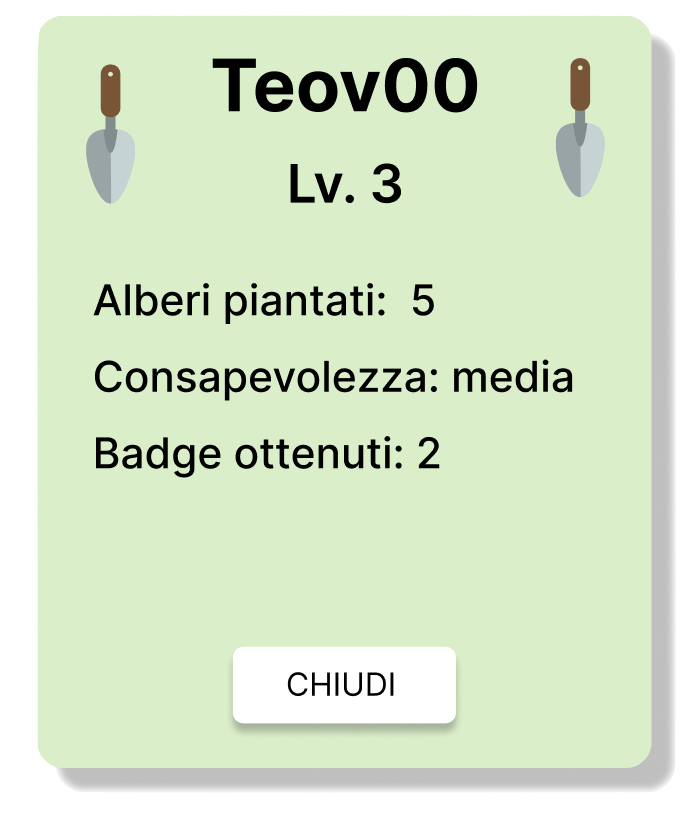
\includegraphics[width=0.30\textwidth]{img/rectDetail.png}
        \label{fig:rectDetail}
    }
    \caption{Tre diversi stili per il pannello dei dettagli nel totem: mensola, tendina e rettangolo}
    \label{fig:detailBanner}
\end{figure}

\begin{figure}[h]
    \centering
    \subfloat[]{
        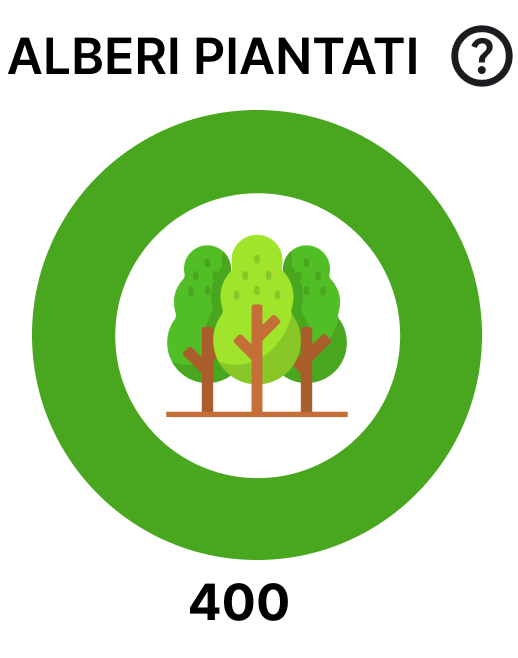
\includegraphics[width=0.3\textwidth]{img/plantedTreeStats.png}
        \label{fig:iconStats}
    }
    \subfloat[]{
        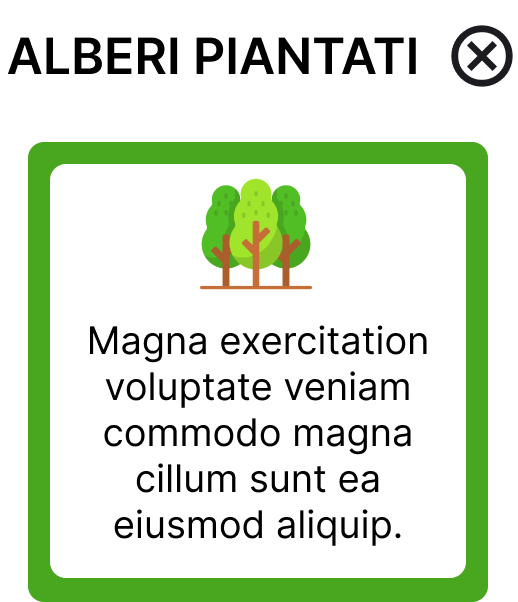
\includegraphics[width=0.3\textwidth]{img/plantedTreeStatsdescr.png}
        \label{fig:descrShowedStats}
    }
    \caption[Pagina delle statistiche nel totem]{Singolo contatore della schermata delle statistiche nel totem. Al tocco del contatore viene mostrata o nascosta la descrizione passando da \ref{fig:iconStats} a \ref{fig:descrShowedStats} e viceversa}
    \label{fig:statCircle}
\end{figure}

\begin{figure}[h]
    \centering
    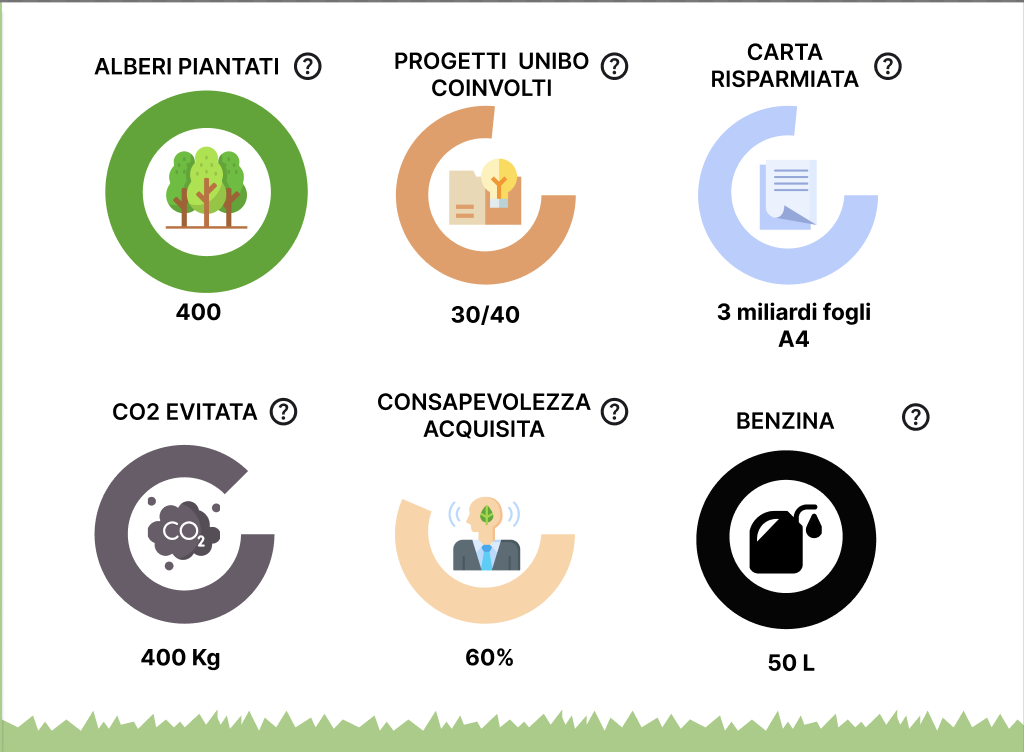
\includegraphics[width=0.8\textwidth]{img/statsPage.png}
    \caption[Pagina delle statistiche nel totem]{Pagina delle statistiche nel totem che presenta sei contatori disposti a griglia}
    \label{fig:statsPage}
\end{figure}

\begin{figure}[h]
    \centering
    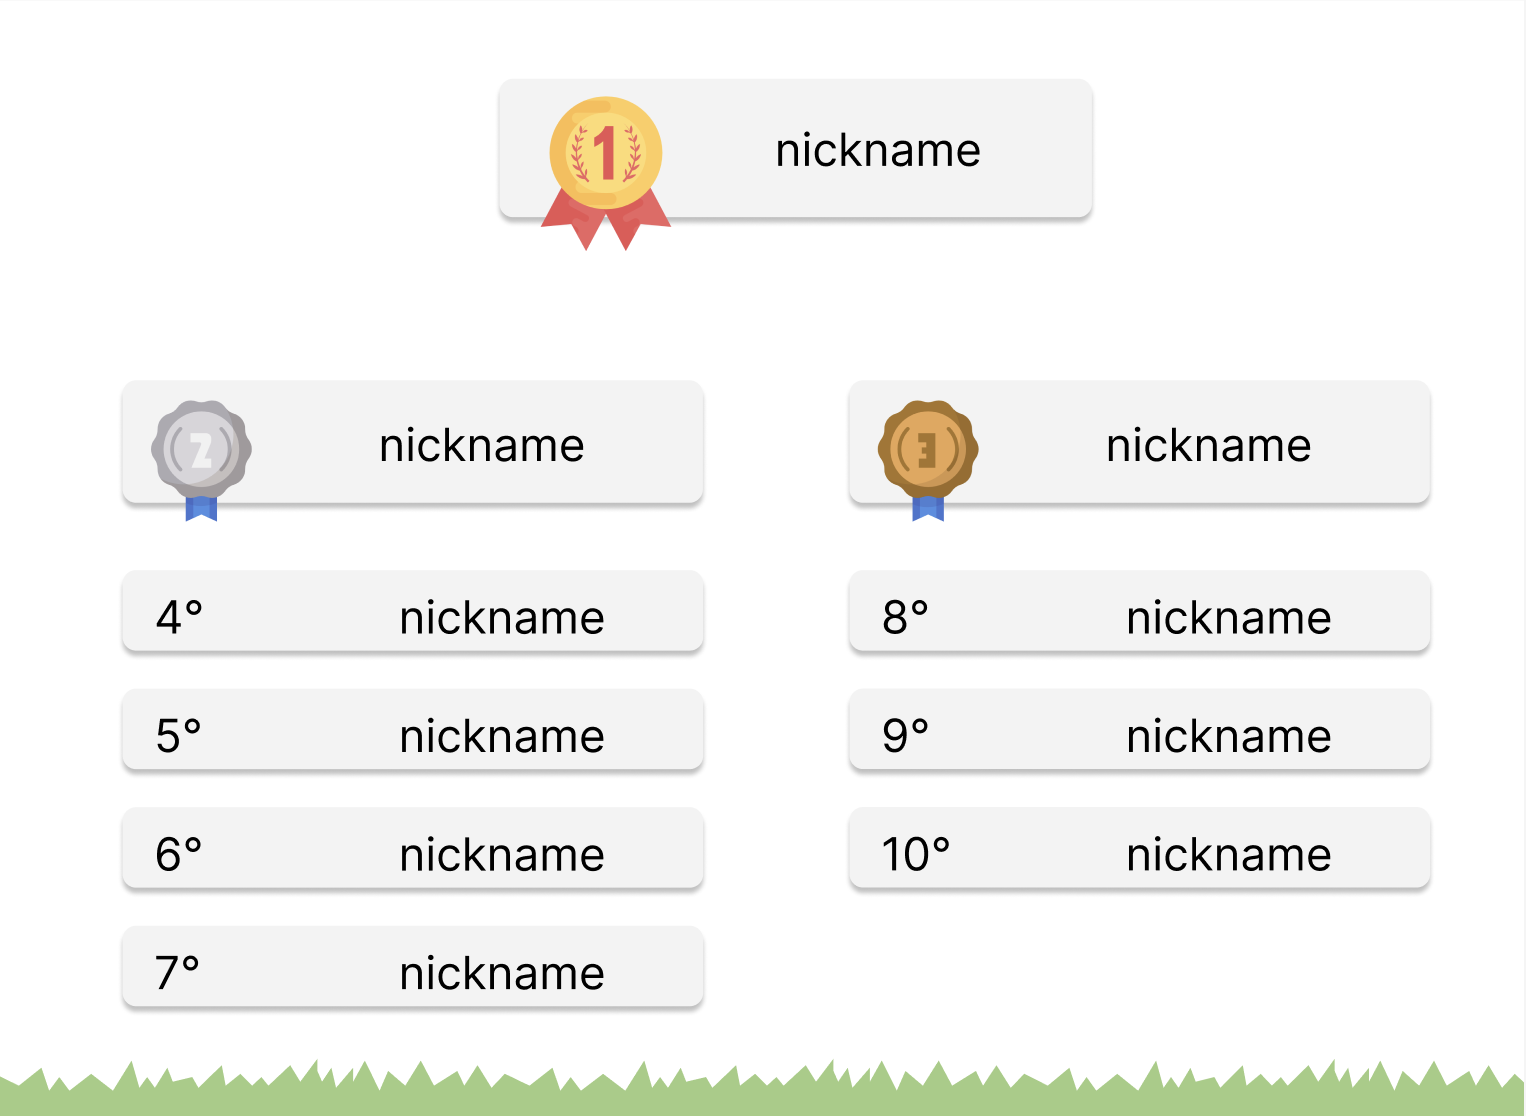
\includegraphics[width=0.8\textwidth]{img/topchartPage.png}
    \caption[Classifica Top10 nel totem]{Pagina della classifica dei 10 migliori utenti}
    \label{fig:chartPage}
\end{figure}

\begin{figure}[h]
    \centering
    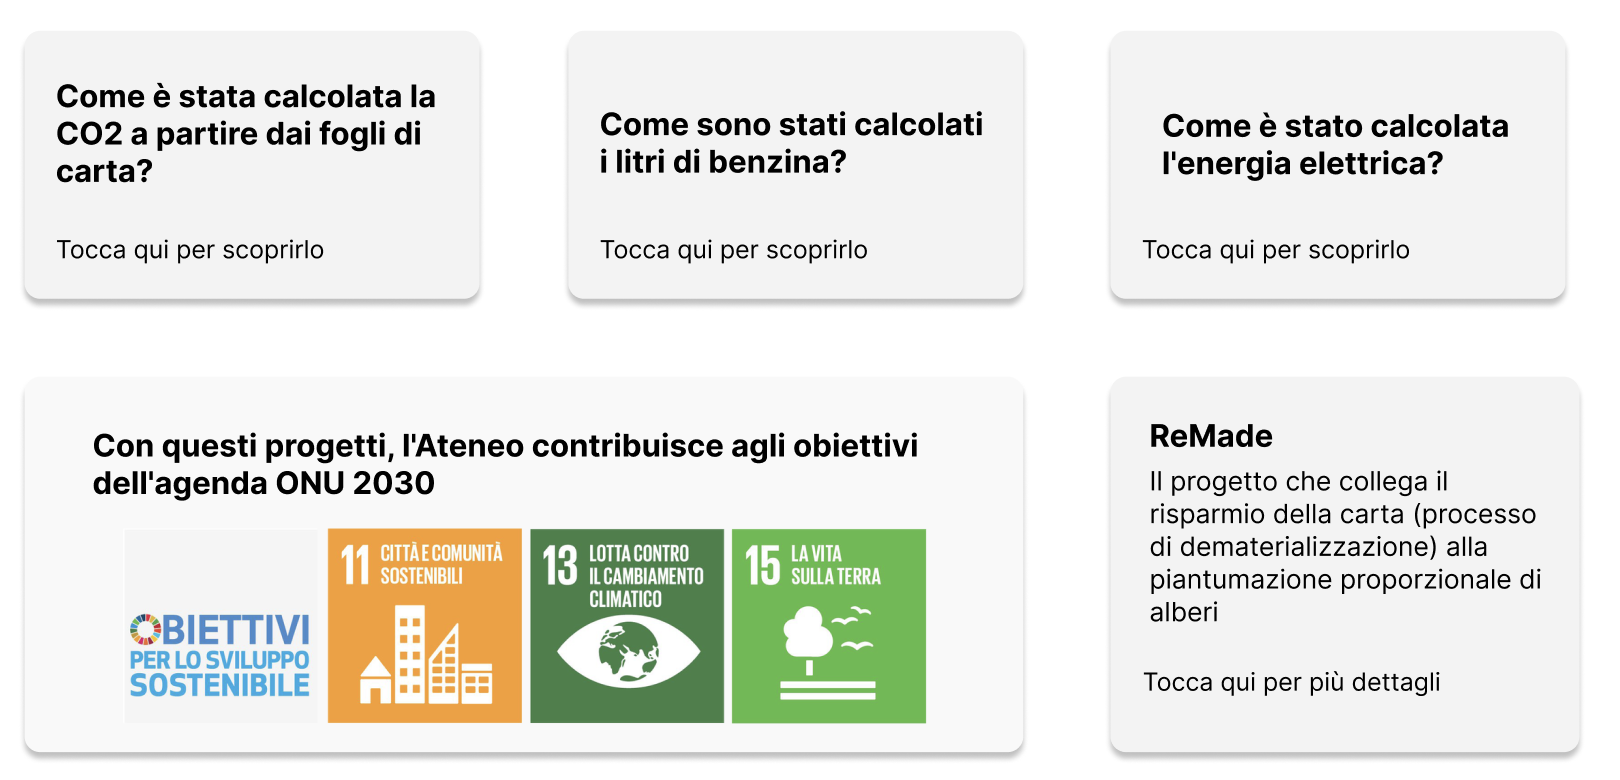
\includegraphics[width=0.8\textwidth]{img/infoPage.png}
    \caption[Pagina delle informazioni nel totem]{Pagina delle informazioni nel totem che prevede un design semplice con delle \textit{tiles} (\enquote*{piastrelle}) disposte a griglia. Al tocco di una tile si apre un pop-up che mostra maggiori informazioni.}
    \label{fig:infoPage}
\end{figure}
\pagebreak
%
%
%
\section{Tecnologie impiegate}
In questo capitolo vengono presentate le tecnologie utilizzate per lo sviluppo della applicativo del totem e della applicazione mobile. Per entrambi i dispositivi si è sviluppato utilizzando il framework Flutter, per l'integrazione e gestione dei dati è stato utilizzato il servizio cloud Firebase Realtime mentre per l'identificazione degli alberi e del totem sono stati utilizzati i codici QR.

\subsection{Flutter}
Flutter \cite{flutter} è un kit di sviluppo software (\textit{Software Development Kit}, SDK) \textit{open source}\footnote{software pubblico alla quale è possibile applicare modifiche, miglioramenti e redistribuirlo liberamente} che comprende diversi strumenti (\textit{DevTools}) per lo sviluppo di applicazioni multi-piattaforma con particolare attenzione alla interfaccia utente (UI, \textit{User Interface}). All'interno del SDK è contenuto il framework Flutter che utilizza il linguaggio di programmazione Dart, anch'esso sviluppato da Google, e librerie grafiche predefinite per le piattaforme Android e iOS.

Il linguaggio Dart è un linguaggio di programmazione ad alto livello multi paradigma, influenzato da altri linguaggi come il C e Java, ed è ottimizzato per lo sviluppo veloce di applicazioni su qualsiasi piattaforma nativa e web.

\subsection{Firebase Realtime}
Firebase Realtime \cite{firebase} è un database non relazionale (NoSQL) memorizzato nel cloud. In quanto NoSQL, i dati e le relazioni non vengono memorizzati in tabelle ma in documenti, archivi \textit{wide-column} o grafi (nodi e archi) a seconda della tipologia del database.
Firebase Realtime è di tipo documentale e quindi fa uso di documenti in formato JSON (\textit{JavaScript Object Notation}) per salvare i dati. Questo genere di memorizzazione permette maggiore flessibilità dello schema permettendo l'aggiunta o la modifica del modello dei dati (es. aggiunta o modifica di un campo). Inoltre i database NoSQL consentono una maggiore velocità e agilità di memorizzazione ed elaborazione oltre che offrire una maggiore scalabilità.
%
\subsection{Codici QR}
Il codice QR (\textit{Quick Response}) è un tipo di codice a barre a matrice (codice 2D) sviluppato e presentato nel 1994 dalla compagnia giapponese Denso Wave che si compone di tanti piccoli quadrati neri e bianchi, chiamati moduli, disposti in una matrice \cite{qrCodeDensoWave}.
I codici QR permettono di memorizzare una quantità variabile di dati che dipende dalla tipologia di dato, dalla versione utilizzata e dal livello di correzione dell'errore. La dimensione della matrice è definita dalla versione utilizzata e anche dalla tipologia di codice QR (Modello 1 o 2, \textit{Micro QR Code}, \textit{rMQR Code}, \textit{SQRC}, Frame QR).

La versione più comune di \textit{QR code} è di tipo \textit{Model 1 o 2} di livello 3, presenta 29x29 moduli ed è in grado di memorizzare fino ad un massimo di 77 caratteri alfanumerici con la correzione dell'errore del 7\% circa.

\section{Strumenti di sviluppo}
\subsection{Git}
Git \cite{gitSite} è un \textit{Version Control System} VCS cioè un sistema di controllo delle versioni dei file. I cambiamenti di uno o più file nel tempo vengono memorizzati e questo permette di mantenere una cronologia dei cambiamenti e di ripristinare una versione precedente di file, cartelle o interi progetti. Esistono diverse tipologie di VCS: locale, centralizzato o distribuito.
Rispetto ai tradizionali VCS, Git non memorizza le differenze dei file (\textit{delta-based version control}) ma memorizza una istantanea di come appaiono i file nel \textit{filesystem} nell'istante in cui si effettua un salvataggio di versione (\textit{commit}). Git considera i suoi dati più come a un flusso d'istantanee del progetto che viene tracciato.

\subsection{Visual Studio Code}
Visual Studio Code \cite{vsCodeSite} è un editor di codice sorgente, sviluppato da Microsoft per Windows, Mac e Linux. Prevede diverse funzionalità utili per la scrittura di codice come la previsione e suggerimento di codice (IntelliSense) e gli strumenti di segnalazione e correzione degli errori, che i comuni editor di testo non possiedono.
Può essere utilizzato con la maggior parte dei linguaggi di programmazione (es. C, Java, PHP) ed è possibile aggiungerne di nuovi ed estendere le sue capacità attraverso dei \textit{plugin} scaricabili direttamente all'interno di Visual Studio Code.
Viste le qualità di questo editor e al suo utilizzo pregresso si è deciso di utilizzarlo per lo sviluppo di questo progetto con l'integrazione del \textit{plugin} ufficiale di Flutter che aggiunge ulteriori strumenti di analisi e \textit{debug}.